\section{Data}

\begin{table}[H]
    \centering
    \caption{Common table for FFT tests, Time(ms)}
    \label{tab:appendix:common:cpp}
    \resizebox{\columnwidth}{!}{
        \rowcolors{1}{}{lightgray}
\begin{tabular}{lrrrr}\toprule
\textbf{Block size}  & \textbf{Columbia Iterative} & \textbf{KISS} & \textbf{Princeton Iterative} & \textbf{Princeton Recursive}\\\midrule
\textbf{16}  & 0.0072 $\pm$ 0.0002 & 0.0056 $\pm$ 0.0002 & 0.0097 $\pm$ 0.0006 & 0.0202 $\pm$ 0.0008\\
\textbf{32}  & 0.0086 $\pm$ 0.0006 & 0.0069 $\pm$ 0.0002 & 0.0132 $\pm$ 0.0002 & 0.0368 $\pm$ 0.0008\\
\textbf{64}  & 0.0083 $\pm$ 0.0008 & 0.0079 $\pm$ 0.0002 & 0.0214 $\pm$ 0.0008 & 0.0705 $\pm$ 0.0022\\
\textbf{128}  & 0.0115 $\pm$ 0.0006 & 0.0131 $\pm$ 0.0006 & 0.0342 $\pm$ 0.0008 & 0.1434 $\pm$ 0.0012\\
\textbf{256}  & 0.0200 $\pm$ 0.0008 & 0.0182 $\pm$ 0.0008 & 0.0627 $\pm$ 0.0008 & 0.2978 $\pm$ 0.0025\\
\textbf{512}  & 0.0366 $\pm$ 0.0006 & 0.0461 $\pm$ 0.0022 & 0.1225 $\pm$ 0.0006 & 0.6379 $\pm$ 0.0035\\
\textbf{1024}  & 0.0773 $\pm$ 0.0020 & 0.0992 $\pm$ 0.0172 & 0.2744 $\pm$ 0.0098 & 1.3437 $\pm$ 0.0086\\
\textbf{2048}  & 0.2604 $\pm$ 0.0123 & 0.2047 $\pm$ 0.0149 & 0.5257 $\pm$ 0.0035 & 2.8773 $\pm$ 0.0253\\
\textbf{4096}  & 0.7974 $\pm$ 0.0216 & 0.4022 $\pm$ 0.0123 & 1.1701 $\pm$ 0.0118 & 6.1206 $\pm$ 0.0598\\
\textbf{8192}  & 1.9326 $\pm$ 0.0519 & 1.2470 $\pm$ 0.0451 & 2.5845 $\pm$ 0.0410 & 13.2345 $\pm$ 0.1433\\
\textbf{16384}  & 4.2789 $\pm$ 0.1254 & 2.3713 $\pm$ 0.0962 & 5.4518 $\pm$ 0.1149 & 27.6080 $\pm$ 0.1784\\
\textbf{32768}  & 9.9388 $\pm$ 0.3203 & 6.7420 $\pm$ 0.2534 & 12.2266 $\pm$ 0.4831 & 55.1227 $\pm$ 1.2277\\
\textbf{65536}  & 23.1031 $\pm$ 0.7648 & 16.0281 $\pm$ 0.3542 & 27.2805 $\pm$ 0.9530 & 102.1585 $\pm$ 3.5262\\
\textbf{131072}  & 75.4942 $\pm$ 1.6429 & 41.7620 $\pm$ 0.5968 & 78.9501 $\pm$ 1.9300 & 231.2663 $\pm$ 6.7357\\
\textbf{262144} & 243.8496 $\pm$ 1.0072 & 102.1196 $\pm$ 1.0817 & 250.4870 $\pm$ 5.2771 & 494.7038 $\pm$ 13.6690\\
\bottomrule
\end{tabular}

    }
\end{table}

\begin{table}[H]
    \centering
    \caption{Common table for Java tests, Time(ms)}
    \label{tab:appendix:common:java}
    \rowcolors{1}{}{lightgray}
\begin{tabular}{lrrr}\toprule
\textbf{Block size}  & \textbf{Columbia Iterative} & \textbf{Princeton Iterative} & \textbf{Princeton Recursive}\\\midrule
\textbf{16}  & 0.03 $\pm$ 0.0010 & 0.12 $\pm$ 0.0053 & 0.13 $\pm$ 0.0108\\
\textbf{32}  & 0.08 $\pm$ 0.0033 & 0.13 $\pm$ 0.1198 & 0.06 $\pm$ 0.0035\\
\textbf{64}  & 0.02 $\pm$ 0.0125 & 0.09 $\pm$ 0.0468 & 0.13 $\pm$ 0.0043\\
\textbf{128}  & 0.01 $\pm$ 0.0002 & 0.14 $\pm$ 0.0020 & 0.49 $\pm$ 0.0486\\
\textbf{256}  & 0.02 $\pm$ 0.0008 & 0.56 $\pm$ 0.0947 & 0.69 $\pm$ 0.0325\\
\textbf{512}  & 0.06 $\pm$ 0.0010 & 0.87 $\pm$ 0.0615 & 1.75 $\pm$ 0.1245\\
\textbf{1024}  & 0.14 $\pm$ 0.0061 & 1.74 $\pm$ 0.0676 & 3.76 $\pm$ 0.2328\\
\textbf{2048}  & 0.43 $\pm$ 0.0159 & 4.40 $\pm$ 0.2064 & 8.69 $\pm$ 0.4575\\
\textbf{4096}  & 1.20 $\pm$ 0.0355 & 9.67 $\pm$ 0.4694 & 25.02 $\pm$ 0.8491\\
\textbf{8192}  & 2.87 $\pm$ 0.0637 & 22.96 $\pm$ 1.1025 & 52.08 $\pm$ 1.3973\\
\textbf{16384}  & 6.32 $\pm$ 0.2066 & 58.38 $\pm$ 1.9484 & 112.30 $\pm$ 1.6050\\
\textbf{32768}  & 12.26 $\pm$ 0.5700 & 150.72 $\pm$ 1.0864 & 239.07 $\pm$ 2.5276\\
\textbf{65536}  & 24.98 $\pm$ 0.9069 & 356.98 $\pm$ 1.5864 & 522.74 $\pm$ 6.1660\\
\textbf{131072}  & 85.94 $\pm$ 1.6097 & 815.86 $\pm$ 3.4304 & 1144.88 $\pm$ 17.8736\\
\textbf{262144} & 274.51 $\pm$ 5.1129 & 2108.07 $\pm$ 27.5366 & 2638.05 $\pm$ 40.5424\\
\bottomrule
\end{tabular}

\end{table}

\begin{table}[H]
    \centering
    \caption{Common table for NEON tests, Time(ms)}
    \label{tab:appendix:common:neon}
    \rowcolors{1}{}{lightgray}
\begin{tabular}{lrr}\toprule
\textbf{Block size}  & \textbf{Iterative} & \textbf{Recursive}\\\midrule
\textbf{16}  & 0.005 $\pm$ 0.0004 & 0.010 $\pm$ 0.0006\\
\textbf{32}  & 0.005 $\pm$ 0.0002 & 0.015 $\pm$ 0.0010\\
\textbf{64}  & 0.005 $\pm$ 0.0002 & 0.018 $\pm$ 0.0014\\
\textbf{128}  & 0.008 $\pm$ 0.0002 & 0.028 $\pm$ 0.0016\\
\textbf{256}  & 0.013 $\pm$ 0.0008 & 0.054 $\pm$ 0.0076\\
\textbf{512}  & 0.034 $\pm$ 0.0006 & 0.096 $\pm$ 0.0014\\
\textbf{1024}  & 0.060 $\pm$ 0.0020 & 0.186 $\pm$ 0.0029\\
\textbf{2048}  & 0.192 $\pm$ 0.0176 & 0.365 $\pm$ 0.0082\\
\textbf{4096}  & 0.365 $\pm$ 0.0161 & 0.808 $\pm$ 0.0200\\
\textbf{8192}  & 1.005 $\pm$ 0.0129 & 1.613 $\pm$ 0.0278\\
\textbf{16384}  & 2.155 $\pm$ 0.0502 & 3.569 $\pm$ 0.0857\\
\textbf{32768}  & 4.789 $\pm$ 0.1543 & 7.600 $\pm$ 0.1878\\
\textbf{65536}  & 9.880 $\pm$ 0.2452 & 16.112 $\pm$ 0.3712\\
\textbf{131072}  & 27.815 $\pm$ 0.7146 & 34.165 $\pm$ 0.4722\\
\textbf{262144} & 63.185 $\pm$ 1.2662 & 74.074 $\pm$ 1.0666\\
\bottomrule
\end{tabular}

\end{table}

% \begin{table}[H]
%     \centering
%     \label{tab:common:table:jni}
%     \caption{Common table for JNI tests, Time(\textmu s)}
%     \resizebox{\columnwidth}{!}{
%         \begin{tabular}{|l|c|c|c|}\hline
\textbf{Block size}  & \textbf{Benchmark convert param to vector} & \textbf{Benchmark with no params} & \textbf{Benchmark with vector as param}\\\hline
\textbf{16}  & 5946.0667 $\pm$ 784.3565 & 2557.1667 $\pm$ 493.7816 & 2979.2333 $\pm$ 96.2158\\\hline
\textbf{32}  & 5600.7333 $\pm$ 191.3485 & 2251.7333 $\pm$ 18.0875 & 2953.1000 $\pm$ 24.5474\\\hline
\textbf{64}  & 5789.9333 $\pm$ 316.5874 & 2274.4000 $\pm$ 20.3493 & 2939.2667 $\pm$ 20.0347\\\hline
\textbf{128}  & 8071.4000 $\pm$ 3161.5874 & 2550.4000 $\pm$ 497.6299 & 3309.0667 $\pm$ 328.8276\\\hline
\textbf{256}  & 7586.8333 $\pm$ 488.9577 & 2295.1667 $\pm$ 22.9024 & 3088.5000 $\pm$ 59.1501\\\hline
\textbf{512}  & 10175.3667 $\pm$ 1575.4113 & 2343.8667 $\pm$ 21.3224 & 3208.3333 $\pm$ 131.3823\\\hline
\textbf{1024}  & 7036.3000 $\pm$ 1666.6088 & 2333.3667 $\pm$ 16.5224 & 4486.2000 $\pm$ 1041.4911\\\hline
\textbf{2048}  & 6954.9333 $\pm$ 976.3683 & 2400.9333 $\pm$ 88.2733 & 3970.4000 $\pm$ 306.6608\\\hline
\textbf{4096}  & 7543.4000 $\pm$ 2469.1806 & 2349.0000 $\pm$ 54.1446 & 4284.7000 $\pm$ 869.9760\\\hline
\textbf{8192}  & 7359.3000 $\pm$ 2058.9155 & 2316.0000 $\pm$ 18.7790 & 3911.4333 $\pm$ 322.5315\\\hline
\textbf{16384}  & 6401.1333 $\pm$ 524.5899 & 2312.4667 $\pm$ 17.3997 & 5355.7333 $\pm$ 631.9348\\\hline
\textbf{32768}  & 10168.4333 $\pm$ 3104.6108 & 2309.0333 $\pm$ 19.1719 & 6260.3000 $\pm$ 1008.9804\\\hline
\textbf{65536} & 12772.4667 $\pm$ 2355.3669 & 1989.6000 $\pm$ 181.0611 & 6064.3333 $\pm$ 675.6516\\\hline
\end{tabular}

%     }
% \end{table}
%
% \begin{table}[H]
%     \centering
%     \label{tab:common:table:cpp}
%     \caption{Common table for C++ tests, Time (ms)}
%     \resizebox{\columnwidth}{!}{
%         \begin{tabular}{|l|c|c|c|c|c|}\hline
\textbf{Block size}  & \textbf{Columbia converted Iterative} & \textbf{Columbia optimized Iterative} & \textbf{KISS} & \textbf{Princeton converted Iterative} & \textbf{Princeton converted Recursive}\\\hline
\textbf{16}  & 0.0225 $\pm$ 0.0033 & 0.0198 $\pm$ 0.0025 & 0.0195 $\pm$ 0.0067 & 0.0342 $\pm$ 0.0053 & 0.0612 $\pm$ 0.0065\\\hline
\textbf{32}  & 0.0322 $\pm$ 0.0025 & 0.0322 $\pm$ 0.0031 & 0.0239 $\pm$ 0.0031 & 0.0545 $\pm$ 0.0043 & 0.1085 $\pm$ 0.0020\\\hline
\textbf{64}  & 0.0525 $\pm$ 0.0014 & 0.0524 $\pm$ 0.0012 & 0.0338 $\pm$ 0.0020 & 0.0847 $\pm$ 0.0059 & 0.2148 $\pm$ 0.0024\\\hline
\textbf{128}  & 0.1025 $\pm$ 0.0033 & 0.0814 $\pm$ 0.0127 & 0.0629 $\pm$ 0.0084 & 0.1328 $\pm$ 0.0029 & 0.4517 $\pm$ 0.0057\\\hline
\textbf{256}  & 0.0925 $\pm$ 0.0178 & 0.0822 $\pm$ 0.0039 & 0.1158 $\pm$ 0.0035 & 0.2807 $\pm$ 0.0073 & 0.9139 $\pm$ 0.0067\\\hline
\textbf{512}  & 0.1709 $\pm$ 0.0267 & 0.1744 $\pm$ 0.0308 & 0.2109 $\pm$ 0.0049 & 0.5486 $\pm$ 0.0253 & 1.9142 $\pm$ 0.0102\\\hline
\textbf{1024}  & 0.3656 $\pm$ 0.0284 & 0.3397 $\pm$ 0.0108 & 0.4072 $\pm$ 0.0086 & 1.1691 $\pm$ 0.0172 & 4.0665 $\pm$ 0.0127\\\hline
\textbf{2048}  & 0.9177 $\pm$ 0.0541 & 0.7402 $\pm$ 0.0190 & 0.8635 $\pm$ 0.0243 & 2.4714 $\pm$ 0.0188 & 8.7235 $\pm$ 0.0725\\\hline
\textbf{4096}  & 1.6737 $\pm$ 0.0461 & 1.9889 $\pm$ 0.0982 & 1.9558 $\pm$ 0.1347 & 5.3867 $\pm$ 0.1000 & 18.3487 $\pm$ 0.1235\\\hline
\textbf{8192}  & 3.7768 $\pm$ 0.1838 & 3.8584 $\pm$ 0.2236 & 3.8499 $\pm$ 0.1603 & 11.7050 $\pm$ 0.5076 & 38.4780 $\pm$ 0.6441\\\hline
\textbf{16384}  & 8.2947 $\pm$ 0.3759 & 8.5556 $\pm$ 0.5672 & 7.8854 $\pm$ 0.2775 & 24.3807 $\pm$ 0.5902 & 80.4920 $\pm$ 0.8228\\\hline
\textbf{32768}  & 19.1886 $\pm$ 1.1809 & 18.5907 $\pm$ 0.9959 & 17.6197 $\pm$ 0.5490 & 52.3713 $\pm$ 1.1313 & 167.3867 $\pm$ 1.5300\\\hline
\textbf{65536} & 42.8520 $\pm$ 1.4120 & 44.2337 $\pm$ 2.4361 & 38.3601 $\pm$ 0.7332 & 112.4273 $\pm$ 1.1197 & 346.7600 $\pm$ 1.9190\\\hline
\end{tabular}

%     }
% \end{table}
%
% \begin{table}[H]
%     \centering
%     \label{tab:common:table:java}
%     \caption{Common table for Java tests, Time (ms)}
%     \resizebox{\columnwidth}{!}{
%         \begin{tabular}{|l|c|c|c|}\hline
\textbf{Block size}  & \textbf{Columbia Iterative} & \textbf{Princeton Iterative} & \textbf{Princeton Recursive}\\\hline
\textbf{16}  & 0.0210 $\pm$ 0.0008 & 0.1738 $\pm$ 0.0368 & 0.2730 $\pm$ 0.0708\\\hline
\textbf{32}  & 0.0429 $\pm$ 0.0018 & 0.0571 $\pm$ 0.0071 & 0.3983 $\pm$ 0.0568\\\hline
\textbf{64}  & 0.0906 $\pm$ 0.0010 & 0.0916 $\pm$ 0.0073 & 0.2104 $\pm$ 0.0402\\\hline
\textbf{128}  & 0.2233 $\pm$ 0.0382 & 0.2353 $\pm$ 0.0339 & 0.3204 $\pm$ 0.0425\\\hline
\textbf{256}  & 0.0372 $\pm$ 0.0022 & 0.4380 $\pm$ 0.0316 & 0.7415 $\pm$ 0.0431\\\hline
\textbf{512}  & 0.0754 $\pm$ 0.0029 & 0.9865 $\pm$ 0.0672 & 1.7743 $\pm$ 0.1944\\\hline
\textbf{1024}  & 0.1507 $\pm$ 0.0059 & 2.0255 $\pm$ 0.0933 & 3.5339 $\pm$ 0.2466\\\hline
\textbf{2048}  & 0.4299 $\pm$ 0.0312 & 4.5366 $\pm$ 0.3038 & 8.2740 $\pm$ 0.6905\\\hline
\textbf{4096}  & 0.9984 $\pm$ 0.0915 & 10.6191 $\pm$ 0.8679 & 17.9445 $\pm$ 0.9022\\\hline
\textbf{8192}  & 2.3125 $\pm$ 0.2709 & 27.5617 $\pm$ 1.9755 & 37.6118 $\pm$ 1.5008\\\hline
\textbf{16384}  & 4.8597 $\pm$ 0.4114 & 62.6869 $\pm$ 1.7191 & 80.1848 $\pm$ 1.9414\\\hline
\textbf{32768}  & 11.2535 $\pm$ 0.9718 & 155.5247 $\pm$ 2.7411 & 172.5062 $\pm$ 2.2489\\\hline
\textbf{65536} & 26.3906 $\pm$ 2.1662 & 366.0557 $\pm$ 2.8910 & 366.6833 $\pm$ 3.3610\\\hline
\end{tabular}

%     }
% \end{table}
%
% \begin{table}[H]
%     \centering
%     \label{tab:jni:convert}
%     \caption{JNI convert, Time (textmu s)}
%     \input{Data/results/JNI/Benchmark_convert.tex}
% \end{table}
%
% \begin{table}[H]
%     \centering
%     \label{tab:jni:no:params}
%     \caption{JNI no parameters, Time (textmu s)}
%     \input{Data/results/JNI/Benchmark_no_params.tex}
% \end{table}
%
% \begin{table}[H]
%     \centering
%     \label{tab:jni:vector}
%     \caption{JNI convert, Time (textmu s)}
%     \input{Data/results/JNI/Benchmark_vector.tex}
% \end{table}
%
% \begin{table}[H]
%     \centering
%     \label{tab:java:princeton:iterative}
%     \caption{Java Princeton Iterative, Time (ms)}
%     /home/algo/Skola/Exjobb/Data/results/FFT/Java_Princeton_Iterative_N_30.tex
% \end{table}
%
% \begin{table}[H]
%     \centering
%     \label{tab:java:princeton:recursive}
%     \caption{Java Princeton Recursive, Time (ms)}
%     \input{Data/results/FFT/Java_Princeton_Recursive.tex}
% \end{table}
%
% \begin{table}[H]
%     \centering
%     \label{tab:java:columbia:iterative}
%     \caption{Java Columbia Iterative, Time (ms)}
%     /home/algo/Skola/Exjobb/Data/results/FFT/Java_Columbia_Iterative_N_30.tex
% \end{table}
%
% \begin{table}[H]
%     \centering
%     \label{tab:cpp:princeton:iterative}
%     \caption{C++ Princeton Iterative, Time (ms)}
%     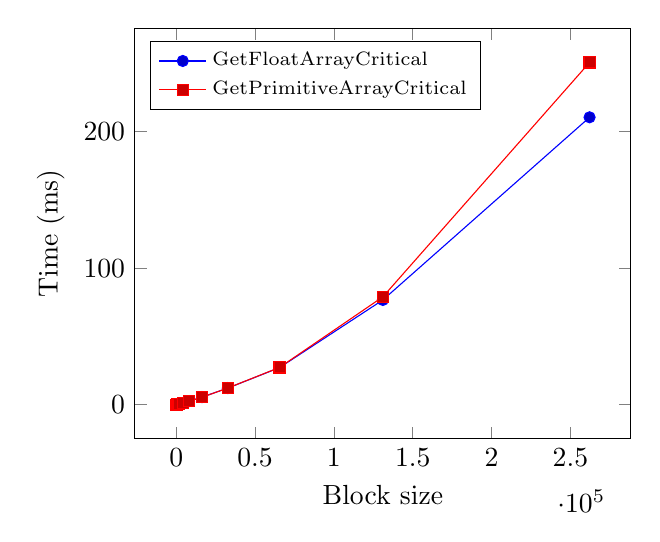
\begin{tikzpicture}
\begin{axis}[xlabel={Block size},ylabel={Time (ms)},width=0.65\linewidth,legend pos=north west,scaled y ticks = false,legend cell align=left,legend style={font=\scriptsize}]
\addplot coordinates {
(16, 0.0083)
(32, 0.0124)
(64, 0.0201)
(128, 0.0348)
(256, 0.0651)
(512, 0.1275)
(1024, 0.2659)
(2048, 0.5235)
(4096, 1.1475)
(8192, 2.6441)
(16384, 5.5785)
(32768, 12.1775)
(65536, 27.1549)
(131072, 76.6735)
(262144, 210.3414)
};
\addplot coordinates {
(16, 0.0097)
(32, 0.0132)
(64, 0.0214)
(128, 0.0342)
(256, 0.0627)
(512, 0.1225)
(1024, 0.2744)
(2048, 0.5257)
(4096, 1.1701)
(8192, 2.5845)
(16384, 5.4518)
(32768, 12.2266)
(65536, 27.2805)
(131072, 78.9501)
(262144, 250.4870)
};
\legend{GetFloatArrayCritical, GetPrimitiveArrayCritical}
\end{axis}
\end{tikzpicture}

% \end{table}
%
% \begin{table}[H]
%     \centering
%     \label{tab:cpp:princeton:recursive}
%     \caption{C++ Princeton Recursive, Time (ms)}
%     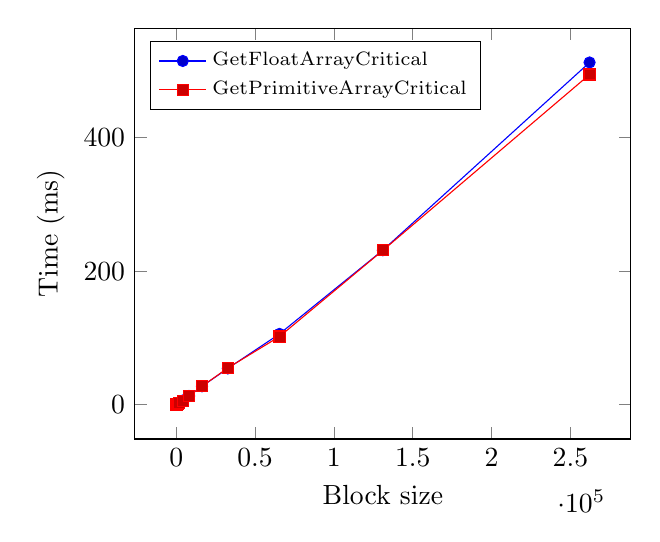
\begin{tikzpicture}
\begin{axis}[xlabel={Block size},ylabel={Time (ms)},width=0.65\linewidth,legend pos=north west,scaled y ticks = false,legend cell align=left,legend style={font=\scriptsize}]
\addplot coordinates {
(16, 0.0187)
(32, 0.0347)
(64, 0.0709)
(128, 0.1447)
(256, 0.3014)
(512, 0.6505)
(1024, 1.3689)
(2048, 2.9279)
(4096, 6.2499)
(8192, 13.1419)
(16384, 27.7314)
(32768, 54.4151)
(65536, 106.1420)
(131072, 231.5323)
(262144, 512.7674)
};
\addplot coordinates {
(16, 0.0202)
(32, 0.0368)
(64, 0.0705)
(128, 0.1434)
(256, 0.2978)
(512, 0.6379)
(1024, 1.3437)
(2048, 2.8773)
(4096, 6.1206)
(8192, 13.2345)
(16384, 27.6080)
(32768, 55.1227)
(65536, 102.1585)
(131072, 231.2663)
(262144, 494.7038)
};
\legend{GetFloatArrayCritical, GetPrimitiveArrayCritical}
\end{axis}
\end{tikzpicture}

% \end{table}
%
% \begin{table}[H]
%     \centering
%     \label{tab:cpp:columbia:iterative}
%     \caption{C++ Columbia Iterative, Time (ms)}
%     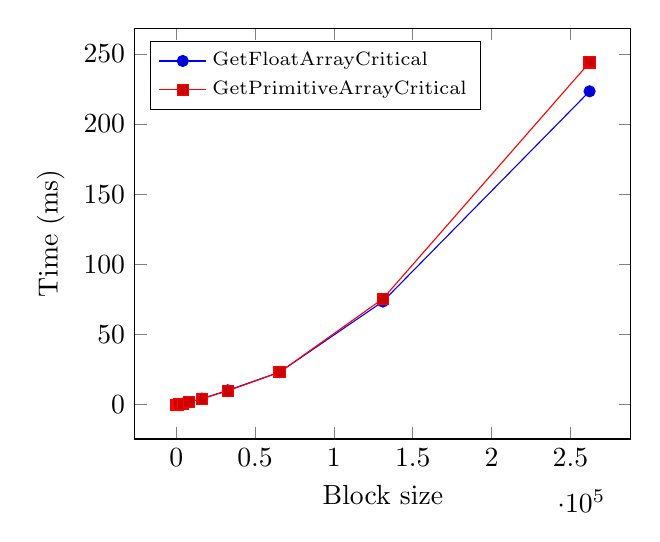
\begin{tikzpicture}
\begin{axis}[xlabel={Block size},ylabel={Time (ms)},width=0.65\linewidth,legend pos=north west,scaled y ticks = false,legend cell align=left,legend style={font=\scriptsize}]
\addplot coordinates {
(16, 0.0057)
(32, 0.0070)
(64, 0.0092)
(128, 0.0136)
(256, 0.0222)
(512, 0.0418)
(1024, 0.0970)
(2048, 0.2761)
(4096, 0.7818)
(8192, 1.8794)
(16384, 4.3304)
(32768, 10.2608)
(65536, 23.1917)
(131072, 73.5225)
(262144, 223.3088)
};
\addplot coordinates {
(16, 0.0072)
(32, 0.0086)
(64, 0.0083)
(128, 0.0115)
(256, 0.0200)
(512, 0.0366)
(1024, 0.0773)
(2048, 0.2604)
(4096, 0.7974)
(8192, 1.9326)
(16384, 4.2789)
(32768, 9.9388)
(65536, 23.1031)
(131072, 75.4942)
(262144, 243.8496)
};
\legend{GetFloatArrayCritical, GetPrimitiveArrayCritical}
\end{axis}
\end{tikzpicture}

% \end{table}
%
% \begin{table}[H]
%     \centering
%     \label{tab:cpp:kiss}
%     \caption{C++ KISS, Time (ms)}
%     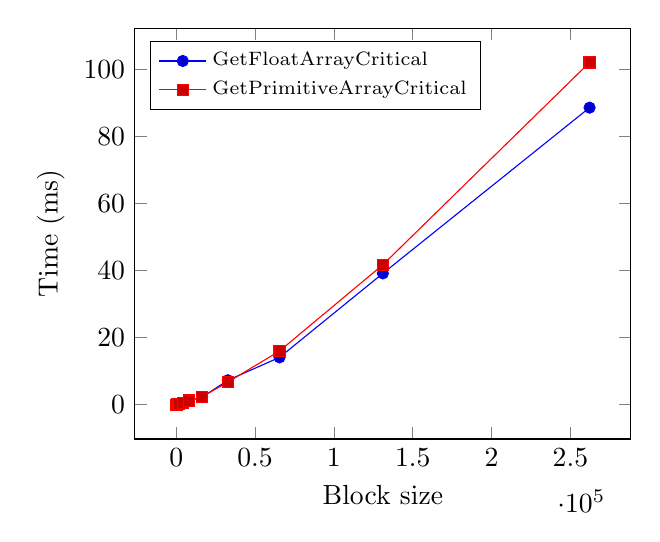
\begin{tikzpicture}
\begin{axis}[xlabel={Block size},ylabel={Time (ms)},width=0.65\linewidth,legend pos=north west,scaled y ticks = false,legend cell align=left,legend style={font=\scriptsize}]
\addplot coordinates {
(16, 0.0050)
(32, 0.0060)
(64, 0.0072)
(128, 0.0139)
(256, 0.0212)
(512, 0.0478)
(1024, 0.0885)
(2048, 0.1965)
(4096, 0.3867)
(8192, 1.1701)
(16384, 2.2685)
(32768, 7.2940)
(65536, 14.1297)
(131072, 39.1887)
(262144, 88.6356)
};
\addplot coordinates {
(16, 0.0056)
(32, 0.0069)
(64, 0.0079)
(128, 0.0131)
(256, 0.0182)
(512, 0.0461)
(1024, 0.0992)
(2048, 0.2047)
(4096, 0.4022)
(8192, 1.2470)
(16384, 2.3713)
(32768, 6.7420)
(65536, 16.0281)
(131072, 41.7620)
(262144, 102.1196)
};
\legend{GetFloatArrayCritical, GetPrimitiveArrayCritical}
\end{axis}
\end{tikzpicture}

% \end{table}
% \begin{table}
%     \centering
%     \label{tab:cpp:columbia:iterative:optimized}
%     \caption{C++ Columbia Iterative Optimized, Time (ms)}
%     \input{Data/results/FFT/CPP_Columbia_optimized.tex}
% \end{table}

% \begin{table}
%     \centering
%     \label{fig:java:columbia:iterative:optimized}
%     \caption{Label here}
%     \input{Data/results/FFT/Java_Columbia_optimized_Iterative.tex}
% \end{table}

% \section{Bar charts}

% \begin{figure}
%     \centering
%     \input{Data/results/FFT/Java_Princeton_Recursive_barchart.tex}
%     \label{fig:java:princeton:recursive:barchart}
%     \caption{Java Princeton Recursive bar chart}
% \end{figure}

\section{ARR}
\begin{figure}[H]
    \centering
    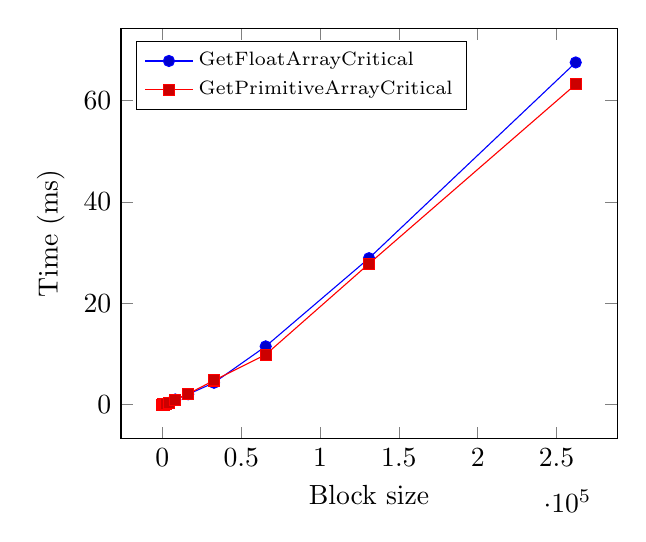
\begin{tikzpicture}
\begin{axis}[xlabel={Block size},ylabel={Time (ms)},width=0.65\linewidth,legend pos=north west,scaled y ticks = false,legend cell align=left,legend style={font=\scriptsize}]
\addplot coordinates {
(16, 0.0045)
(32, 0.0048)
(64, 0.0055)
(128, 0.0087)
(256, 0.0137)
(512, 0.0312)
(1024, 0.0667)
(2048, 0.1327)
(4096, 0.3437)
(8192, 1.0274)
(16384, 2.0687)
(32768, 4.3371)
(65536, 11.5128)
(131072, 28.9012)
(262144, 67.5020)
};
\addplot coordinates {
(16, 0.0057)
(32, 0.0050)
(64, 0.0056)
(128, 0.0089)
(256, 0.0134)
(512, 0.0348)
(1024, 0.0608)
(2048, 0.1925)
(4096, 0.3656)
(8192, 1.0051)
(16384, 2.1559)
(32768, 4.7898)
(65536, 9.8807)
(131072, 27.8158)
(262144, 63.1858)
};
\legend{GetFloatArrayCritical, GetPrimitiveArrayCritical}
\end{axis}
\end{tikzpicture}

    \caption{}
    \label{fig:arr:neon:Iterative}
\end{figure}
\begin{figure}[H]
    \centering
    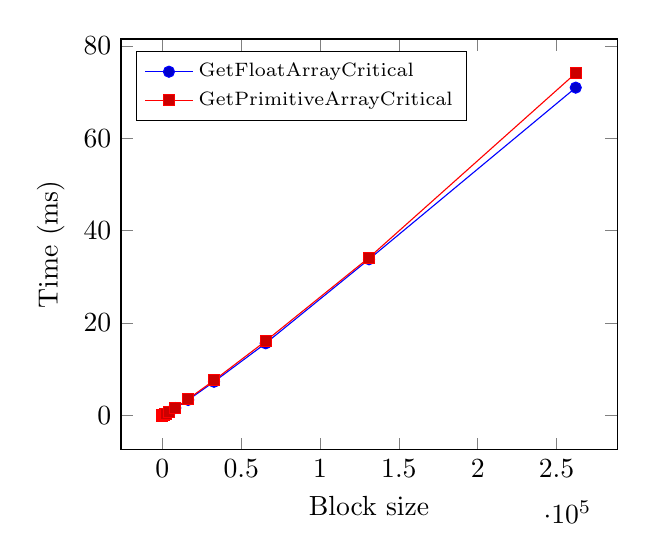
\begin{tikzpicture}
\begin{axis}[xlabel={Block size},ylabel={Time (ms)},width=0.65\linewidth,legend pos=north west,scaled y ticks = false,legend cell align=left,legend style={font=\scriptsize}]
\addplot coordinates {
(16, 0.0079)
(32, 0.0106)
(64, 0.0162)
(128, 0.0280)
(256, 0.0506)
(512, 0.1036)
(1024, 0.1917)
(2048, 0.3825)
(4096, 0.7539)
(8192, 1.6084)
(16384, 3.3681)
(32768, 7.3011)
(65536, 15.6232)
(131072, 33.8117)
(262144, 70.9477)
};
\addplot coordinates {
(16, 0.0108)
(32, 0.0150)
(64, 0.0187)
(128, 0.0286)
(256, 0.0544)
(512, 0.0961)
(1024, 0.1868)
(2048, 0.3659)
(4096, 0.8086)
(8192, 1.6133)
(16384, 3.5690)
(32768, 7.6009)
(65536, 16.1129)
(131072, 34.1650)
(262144, 74.0746)
};
\legend{GetFloatArrayCritical, GetPrimitiveArrayCritical}
\end{axis}
\end{tikzpicture}

    \caption{}
    \label{fig:arr:neon:Recursive}
\end{figure}
\begin{figure}[H]
    \centering
    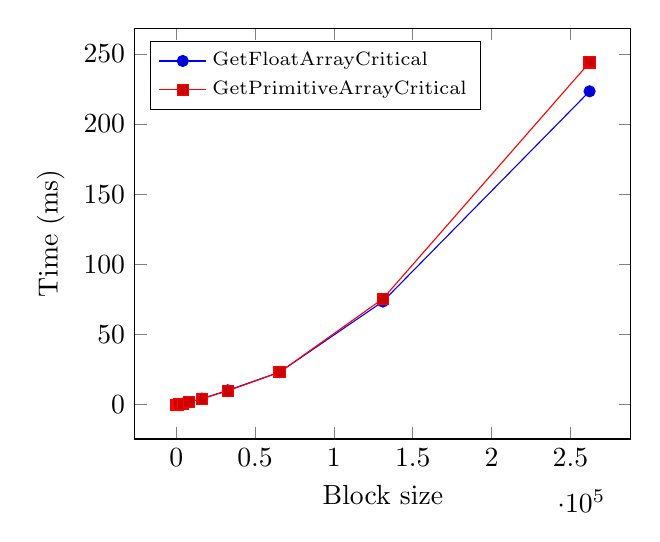
\begin{tikzpicture}
\begin{axis}[xlabel={Block size},ylabel={Time (ms)},width=0.65\linewidth,legend pos=north west,scaled y ticks = false,legend cell align=left,legend style={font=\scriptsize}]
\addplot coordinates {
(16, 0.0057)
(32, 0.0070)
(64, 0.0092)
(128, 0.0136)
(256, 0.0222)
(512, 0.0418)
(1024, 0.0970)
(2048, 0.2761)
(4096, 0.7818)
(8192, 1.8794)
(16384, 4.3304)
(32768, 10.2608)
(65536, 23.1917)
(131072, 73.5225)
(262144, 223.3088)
};
\addplot coordinates {
(16, 0.0072)
(32, 0.0086)
(64, 0.0083)
(128, 0.0115)
(256, 0.0200)
(512, 0.0366)
(1024, 0.0773)
(2048, 0.2604)
(4096, 0.7974)
(8192, 1.9326)
(16384, 4.2789)
(32768, 9.9388)
(65536, 23.1031)
(131072, 75.4942)
(262144, 243.8496)
};
\legend{GetFloatArrayCritical, GetPrimitiveArrayCritical}
\end{axis}
\end{tikzpicture}

    \caption{}
    \label{fig:arr:columbia}
\end{figure}
\begin{figure}[H]
    \centering
    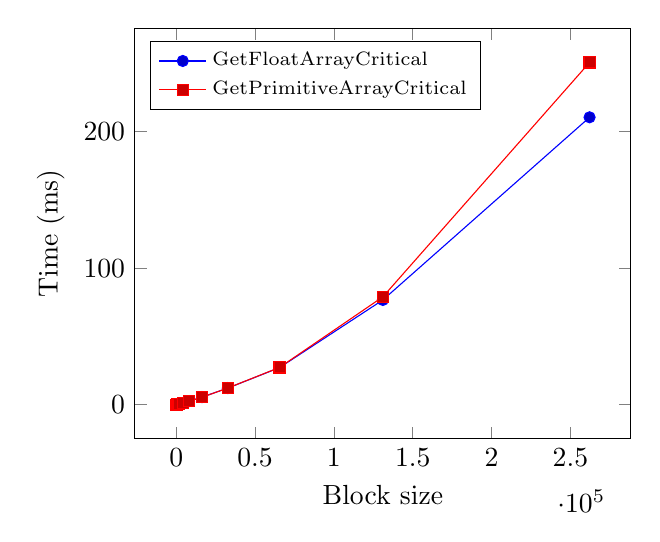
\begin{tikzpicture}
\begin{axis}[xlabel={Block size},ylabel={Time (ms)},width=0.65\linewidth,legend pos=north west,scaled y ticks = false,legend cell align=left,legend style={font=\scriptsize}]
\addplot coordinates {
(16, 0.0083)
(32, 0.0124)
(64, 0.0201)
(128, 0.0348)
(256, 0.0651)
(512, 0.1275)
(1024, 0.2659)
(2048, 0.5235)
(4096, 1.1475)
(8192, 2.6441)
(16384, 5.5785)
(32768, 12.1775)
(65536, 27.1549)
(131072, 76.6735)
(262144, 210.3414)
};
\addplot coordinates {
(16, 0.0097)
(32, 0.0132)
(64, 0.0214)
(128, 0.0342)
(256, 0.0627)
(512, 0.1225)
(1024, 0.2744)
(2048, 0.5257)
(4096, 1.1701)
(8192, 2.5845)
(16384, 5.4518)
(32768, 12.2266)
(65536, 27.2805)
(131072, 78.9501)
(262144, 250.4870)
};
\legend{GetFloatArrayCritical, GetPrimitiveArrayCritical}
\end{axis}
\end{tikzpicture}

    \caption{}
    \label{fig:arr:princeton:iterative}
\end{figure}
\begin{figure}[H]
    \centering
    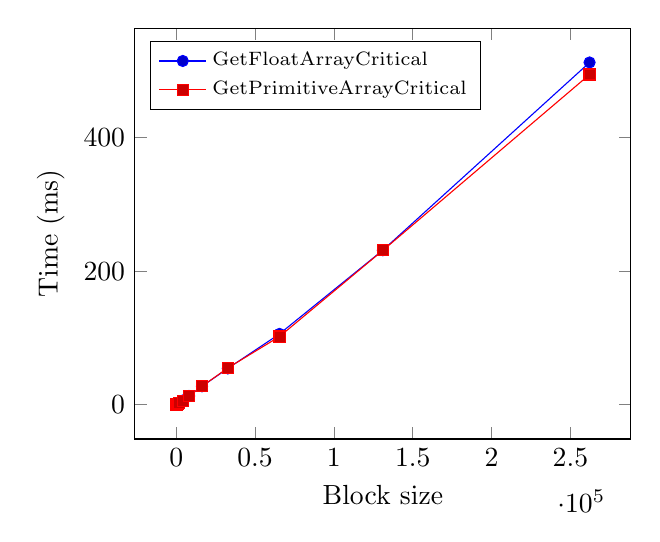
\begin{tikzpicture}
\begin{axis}[xlabel={Block size},ylabel={Time (ms)},width=0.65\linewidth,legend pos=north west,scaled y ticks = false,legend cell align=left,legend style={font=\scriptsize}]
\addplot coordinates {
(16, 0.0187)
(32, 0.0347)
(64, 0.0709)
(128, 0.1447)
(256, 0.3014)
(512, 0.6505)
(1024, 1.3689)
(2048, 2.9279)
(4096, 6.2499)
(8192, 13.1419)
(16384, 27.7314)
(32768, 54.4151)
(65536, 106.1420)
(131072, 231.5323)
(262144, 512.7674)
};
\addplot coordinates {
(16, 0.0202)
(32, 0.0368)
(64, 0.0705)
(128, 0.1434)
(256, 0.2978)
(512, 0.6379)
(1024, 1.3437)
(2048, 2.8773)
(4096, 6.1206)
(8192, 13.2345)
(16384, 27.6080)
(32768, 55.1227)
(65536, 102.1585)
(131072, 231.2663)
(262144, 494.7038)
};
\legend{GetFloatArrayCritical, GetPrimitiveArrayCritical}
\end{axis}
\end{tikzpicture}

    \caption{}
    \label{fig:arr:princeton:recursive}
\end{figure}
\begin{figure}[H]
    \centering
    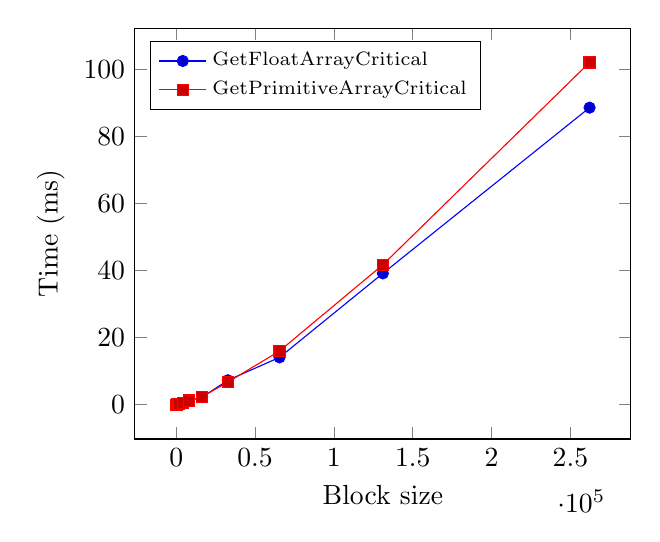
\begin{tikzpicture}
\begin{axis}[xlabel={Block size},ylabel={Time (ms)},width=0.65\linewidth,legend pos=north west,scaled y ticks = false,legend cell align=left,legend style={font=\scriptsize}]
\addplot coordinates {
(16, 0.0050)
(32, 0.0060)
(64, 0.0072)
(128, 0.0139)
(256, 0.0212)
(512, 0.0478)
(1024, 0.0885)
(2048, 0.1965)
(4096, 0.3867)
(8192, 1.1701)
(16384, 2.2685)
(32768, 7.2940)
(65536, 14.1297)
(131072, 39.1887)
(262144, 88.6356)
};
\addplot coordinates {
(16, 0.0056)
(32, 0.0069)
(64, 0.0079)
(128, 0.0131)
(256, 0.0182)
(512, 0.0461)
(1024, 0.0992)
(2048, 0.2047)
(4096, 0.4022)
(8192, 1.2470)
(16384, 2.3713)
(32768, 6.7420)
(65536, 16.0281)
(131072, 41.7620)
(262144, 102.1196)
};
\legend{GetFloatArrayCritical, GetPrimitiveArrayCritical}
\end{axis}
\end{tikzpicture}

    \caption{}
    \label{fig:arr:kiss}
\end{figure}
